\section{The vertex sampling problem}
\label{sec:sampling}

This section rests entirely on the deployed table and the deployed folded
result. No rebuilt table is used, so none of it depends on trusting a
second calculation.

\subsection{What the fold asks for}

The FK two-point fold evaluates the driving-field three-point cumulant on
the collapsed configuration: two directions coincident, the third displaced
by the plotted separation $\gamma$. In the cosine coordinates the vertex
table is indexed by, that is the family $(1,\cos\gamma,\cos\gamma)$. This
was established from the code rather than the documentation, by wrapping
the production callable in a logging shim and running the production
configuration. Across 1\,990\,656 recorded evaluations the fold requests
exactly one sorted cosine triple per separation, and the three leg times
agree to $2\times10^{-13}$, confirming the equal-time collapse. That is the
object \code{sections/appendix.tex} defines in appendix
\emph{append: driving-field spectra}.

\subsection{Where the table has samples}

The deployed table is built on a uniform mesh of 15 cosines, spacing
$1/7$, triangle filtered to 1671 rows, which the callable canonicalises to
351 unique sorted triples. On the collapsed family the mesh therefore has
samples at
\[
  c=1 \;\;(\gamma = 0), \qquad
  c=6/7 \;\;(\gamma = 31.0^\circ = 1860'), \qquad
  c=5/7 \;\;(\gamma = 44.4^\circ), \;\ldots
\]
There is no sample between $\gamma=0$ and $\gamma=1860'$. The figures plot
$0.5'$ to $5000'$, that is $0.008^\circ$ to $83^\circ$. Thirty-five of the
forty plotted separations lie inside the first mesh gap.

The compression is worse than the gap width suggests, because the
interpolation variable is $\cos\gamma$ and $1-\cos\gamma \simeq
\gamma^2/2$. Measured as a fraction of the first interval $[6/7,1]$, the
plotted separations sit at $0.0000\%$ ($\gamma=0.5'$), $0.014\%$
($21.9'$), $0.62\%$ ($144.7'$) and $4.1\%$ ($372.2'$). Twenty-six of the
forty are within $1\%$ of the $c=1$ endpoint. Both endpoints of the
interval are exact table entries; the difficulty is that the plotted range
does not span the interval, it hides inside one end of it.

\subsection{The plotted curve is the interpolation weight}

The callable looks a query up with a \code{cKDTree} over the 351 unique
triples, taking the four nearest neighbours with inverse-distance weights.
Reconstructing that lookup and reading off the normalised weight the rule
places on the $(1,1,1)$ node gives a curve that can be compared directly
with the published FK curve, normalised to its own value at $0.5'$.

They are the same curve. Over the whole range in which the corner node is
in the neighbour set, $0.5'$ to $1535'$, the largest absolute difference is
$5.2\times10^{-5}$ and the largest relative difference is
$2.4\times10^{-4}$ (Figure~\ref{fig:weight}). The plotted angular
dependence of the FK term is the interpolator's weight function. No
property of the vertex enters it.

At $\gamma=1944'$ the corner node leaves the four-neighbour set altogether,
its weight becoming exactly zero, and the curve changes sign. That is
$32.4^\circ$, and it is the feature the caption of Figure~15 in
\code{sections/appendix.tex} describes as ``the sign change at
$\gamma\simeq32^\circ$''. The four neighbours that replace it are
$(1,\tfrac67,\tfrac67)$, $(\tfrac67,\tfrac67,\tfrac67)$,
$(1,\tfrac57,\tfrac57)$ and $(\tfrac67,\tfrac67,\tfrac57)$: one collapsed
configuration at $31^\circ$, one equilateral triangle and one scalene
triangle. The sign change is a change of neighbour set.

\begin{figure}[t]
\centering
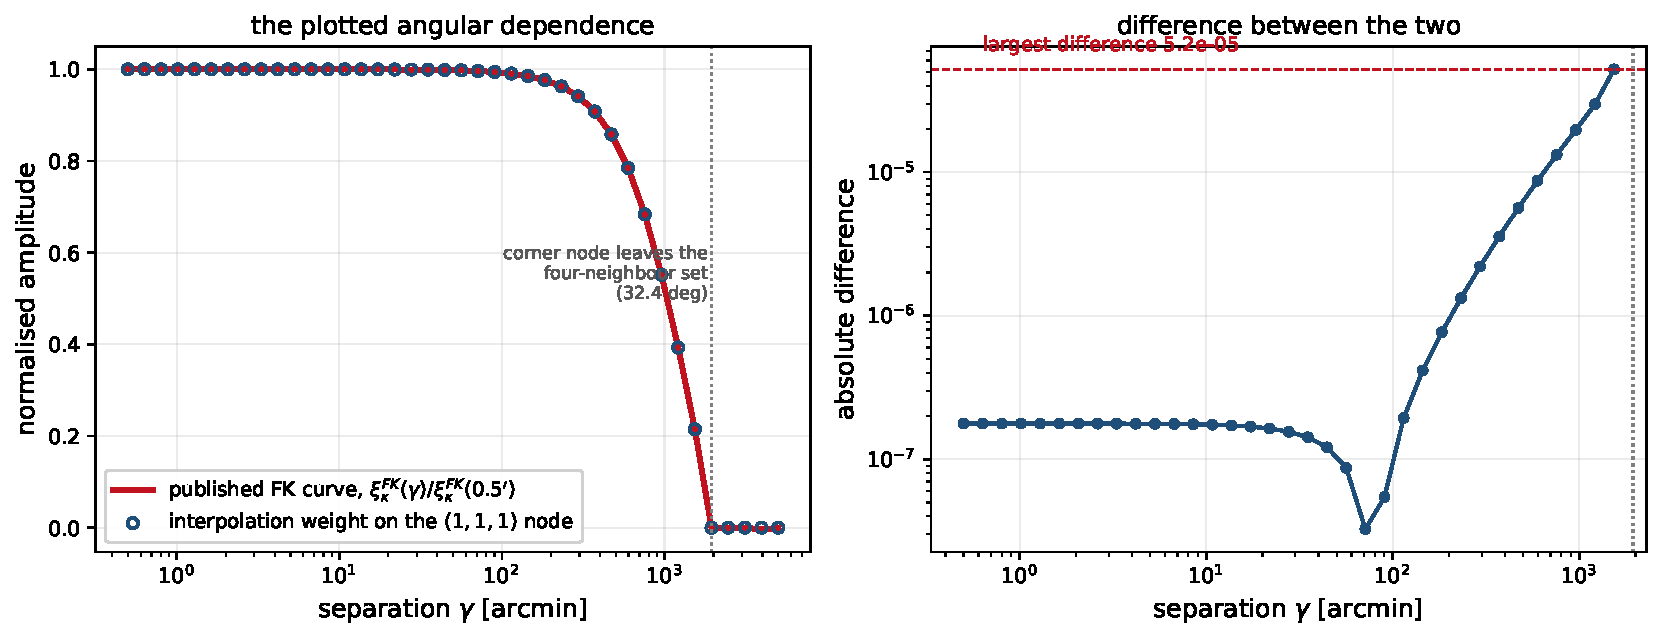
\includegraphics[width=\textwidth]{figures/weight_identity.pdf}
\caption{Left: the published FK curve for $\xi_\kappa$, normalised to its
value at $\gamma=0.5'$, against the normalised inverse-distance weight the
vertex callable places on the $(1,1,1)$ node. Right: the difference between
them. Both come from deployed artefacts only. The dotted line marks the
separation at which the corner node leaves the four-neighbour set, which is
where the published curve changes sign. Produced by
\code{code/rebuild/probe\_weight\_identity.py}.}
\label{fig:weight}
\end{figure}

\subsection{The deployed table's own next sample}

The table also says, by itself, that the vertex cannot be flat across this
range. On the source shell its collapsed-family entries read
$-1.35\times10^{-14}$ at $c=1$ and roughly three orders of magnitude
smaller, with the opposite sign, at $c=6/7$. The deployed file therefore
records that the vertex falls by more than three orders of magnitude and
changes sign somewhere inside the first gap. What it cannot record is
where.

There is an independent reason to expect the decay, which needs no table at
all. The collapsed configuration is the driving-field cumulant with two
points coincident and the third displaced transversely by $r_\perp =
\chi\gamma$ on the same shell. At the mid shell, $\gamma=0.5'$ is
$r_\perp\simeq1$ Mpc while $\gamma=145'$ is $r_\perp\simeq280$ Mpc. Matter
correlations die well before 280 Mpc, so the vertex must decay across the
plotted range. In the same units the mesh spacing of $1/7$ in $\cos\gamma$
is a resolution of about 3600 Mpc in $r_\perp$, while the physics happens
between 1 and 100 Mpc.

\subsection{The draft already contains the counterexample}

Figure~7 of the draft, \code{zeta\_driving\_field\_slices\_draft.pdf}, is
generated from \code{ell\_band\_decomp\_results.npz}, which evaluates the
vertex on the collapsed family at 28 separations directly, with no cosine
mesh and no interpolation. It shows the vertex decaying steeply and
changing sign inside the range over which the FK figures show it flat. The
two figures in the same paper disagree, and the resolved one is right.

\subsection{A second, smaller defect in the same callable}

The callable sorts a query triple descending before lookup and then fills
the coupling tensor with the retrieved value in every index permutation.
Whether that is legitimate depends on the channel. Building the same
collapsed configuration in the two leg orderings that canonicalise to the
same sorted triple, and comparing, gives the median relative differences in
Table~\ref{tab:perm}.

\begin{table}[h]
\centering
\begin{tabular}{lcc}
\toprule
channel & median relative difference & symmetric \\
\midrule
$\zeta_{TTT}$  & $3.3\times10^{-3}$ & yes \\
$\zeta_{Bmod}$ & $3.3\times10^{-3}$ & yes \\
$\zeta_{PPP}$  & $4.9\times10^{-2}$ & no \\
$\zeta_{TPP}$  & $2.3\times10^{-1}$ & no \\
$\zeta_{TTP}$  & $5.9\times10^{-1}$ & no \\
$\zeta_{Dmod}$ & $7.0\times10^{-1}$ & no \\
\bottomrule
\end{tabular}
\caption{Sensitivity of each vertex channel to which leg carries the
offset, over separations up to $200'$. The two orderings canonicalise to
the same sorted triple, so the callable cannot distinguish them and the
difference bounds the error its symmetric fill makes. Maxima are not quoted
because every channel passes through zero in this range. Produced by
\code{code/rebuild/probe\_permutation.py}.}
\label{tab:perm}
\end{table}

The channels that carry $\xi_\kappa$ and $\xi_+$ are symmetric to the
quadrature level, so the symmetric fill costs those two observables
nothing. The channels that enter $\xi_-$ and $\xi_{\kappa\gamma}$ are not,
so those two can be quoted here as magnitudes and signs but not as precise
values. This did not affect the deployed numbers, because the deployed
lookup is pinned at $(1,1,1)$, which has no permutation duplicates. It
becomes live exactly when the grid is refined, which is why it is fixed
rather than merely noted: Section~\ref{sec:callablefix} reports the
correction and what it changes.
